\documentclass[masters]{ucbthesis} %Sets the default text size to 11pt and class to article.
%------------------------Dimensions--------------------------------------------
\topmargin=0.0in %length of margin at the top of the page (1 inch added by default)
\oddsidemargin=0.0in %length of margin on sides for odd pages
\evensidemargin=0in %length of margin on sides for even pages
\textwidth=6.5in %How wide you want your text to be
\marginparwidth=0.5in
\headheight=0pt %1in margins at top and bottom (1 inch is added to this value by default)
\headsep=0pt %Increase to increase white space in between headers and the top of the page
\textheight=9.1in %How tall the text body is allowed to be on each page

\usepackage{url}
\usepackage{algorithmic}
\usepackage{algorithm}
\usepackage{listings}
\usepackage{balance}
\usepackage{graphicx}
\usepackage{hyperref}
% \usepackage{draftwatermark}
% \SetWatermarkText{DRAFT}
% \SetWatermarkScale{5}
% "define" Scala
\lstdefinelanguage{scala}{morekeywords={class,object,trait,extends,with,new,if,while,for,def,val,var,this},
otherkeywords={->,=>},
sensitive=true,
morecomment=[l]{//},
morecomment=[s]{/*}{*/},
morestring=[b]"}
% Default settings for code listings
\lstset{frame=tb,language=scala,aboveskip=3mm,belowskip=3mm,showstringspaces=false,columns=flexible,basicstyle={\small\ttfamily}}
\usepackage{amsmath}

\begin{document}

\title{Scalable Genome Resequencing with \texttt{ADAM} and \texttt{avocado}}
\author{Frank Austin Nothaft}
\degreesemester{Spring}
\degreeyear{2015}
\degree{Master of Science}
\chair{Professor David Patterson}
\othermembers{Professor Anthony Joseph \\
Assistant Professor Nir Yosef}
\numberofmembers{3}
% Previous degrees are no longer to be listed on the title page.
% \prevdegrees{B.A. (University of Northern South Dakota at Hoople) 1978 \\
%   M.S. (Ed's School of Quantum Mechanics and Muffler Repair) 1989}
\field{Computer Science}
% Designated Emphasis -- this is optional, and rare
% \emphasis{Colloidal Telemetry}
% This is optional, and rare
% \jointinstitution{University of Western Maryland}
% This is optional
\campus{Berkeley}

\maketitle

\approvalpage
\copyrightpage

\begin{abstract}
The decreased cost of genome sequencing technologies has made genome sequencing a viable
tool for clinical and populations genomics applications. The efficiency of genome sequencing has
been further improved through large projects like the Human Genome Project, which have assembled
reference genomes for medically/agriculturally important organisms. These reference quality assemblies
have enabled the creation of \emph{genome resequencing pipelines}, where the genome of a single
sample is computed by computing the \emph{difference} between a given sample and the reference
genome for the organism.

While sequencing cost has decreased by more than 10,000$\times$ since the Human Genome Project
concluded in 2003, resequencing pipelines have struggled to keep pace with the growing volume of
genomic data. These tools suffer from limited parallelism because they were not designed to use parallel
or distributed computing techniques, and are limited by asymptotically inefficient algorithms. In this thesis,
we introduce two tools, \texttt{ADAM} and \texttt{avocado}. \texttt{ADAM} provides an efficient framework
for performing distributed genomic analyses, and \texttt{avocado} implements efficient local reassembly
to discover genomic variants.
\end{abstract}

\tableofcontents

\chapter{Introduction}

Since the completion of the Human Genome Project in 2003, genome sequencing costs have dropped
by more than $10,000\times$~\cite{nhgri}. The rapidly declining cost of sequencing a single human
genome has enabled large sequencing projects like the 1000 Genomes Project~\cite{siva08} and
the Cancer Genome Atlas~(TCGA,~\cite{weinstein13}). As these large sequencing projects perform
analysis that process terabytes~(TB) to petabytes~(PB) of genomic data, they have created a demand
for genomic analysis tools that can efficiently process these scales of data~\cite{schadt10, stein10}.

Over a similar time range, commercial needs led to the development of horizontally scalable analytics
systems. The development and deployment of MapReduce at Google~\cite{dean04, dean08} spawned
the development of a variety of distributed analytics tools and the Hadoop ecosystem~\cite{hadoop}.
In turn, these systems led to other systems that provided a more fluent programming
model~\cite{yu08} and higher performance~\cite{zaharia10}. The demand for these systems has
been driven by the increase in the amount of data available to analysts, and has coincided with the
development of statistical systems that are accessible to non-experts, such as
\texttt{Scikit-learn}~\cite{pedregosa11} and \texttt{MLI}~\cite{sparks13}.

With the rapid drop in the cost of sequencing a genome, and the accompanying growth in available data,
there is a good opportunity to apply modern, horizontally scalable analytics systems to genomics. New
projects such as the 100K for UK, which aims to sequence the genomes of 100,000 individuals in the
United Kingdom~\cite{uk100k} will generate three to four \emph{orders of magnitude} more data than
prior projects like the 1000 Genomes Project~\cite{siva08}. These projects use the current ``best
practice'' genomic variant calling pipelines~\cite{auwera13}, which take approximately 120 hours to
process a single, high-quality human genome using a single, beefy node~\cite{talwalkar14}. To address
these challenges, scientists have started to apply computer systems techniques such as
MapReduce~\cite{langmead09, mckenna10, schatz09} and columnar storage~\cite{fritz11} to custom
scientific compute/storage systems. While these systems have improved analysis cost and performance,
current implementations incur significant overheads imposed by the legacy formats and codebases that
they use.

In this thesis, we demonstrate \texttt{ADAM}, a genomic data processing and storage system built using
Apache Avro, Parquet, and Spark~\cite{avro, parquet, zaharia10}, and \texttt{avocado}, a variant caller
built on top of \texttt{ADAM}. This pipeline achieves a 50$\times$ increase in throughput over the current
best practice pipeline, while reducing analysis cost by 50\%. In the process of creating \texttt{ADAM},
we developed a ``narrow waisted'' layering model for building scientific analysis systems. This narrow
waisted stack is inspired by the OSI model for networked systems~\cite{zimmermann80}. However, in our
stack model, the data schema is the narrow waist that separates data processing from data storage. Our
stack solves the following three problems that are common across current scientific analysis systems:

\begin{enumerate}
\item Current scientific systems improve the performance of common patterns by changing the data
model (often by requiring data to be stored in a coordinate-sorted order).
\item Legacy data formats were not designed with horizontal scalability in mind.
\item The system must be able to efficiently access shared metadata, and to slice datasets for running
targeted analyses.
\end{enumerate}

We solve these problems with the following techniques:

\begin{enumerate}
\item We make a schema the ``narrow waist'' of our stack to enforce data independence and
devise algorithms for making common genomics patterns fast.
\item To improve horizontal scalability, we use Parquet, a modern parallel columnar store based off of
Dremel~\cite{melnik10} to push computation to the data.
\item We use a denormalized schema to achieve O(1) parallel access to metadata.
\end{enumerate}

We introduce the stack model in figure~\ref{fig:stack-model} as a way to decompose scientific systems.

\begin{figure}[h]
\begin{center}
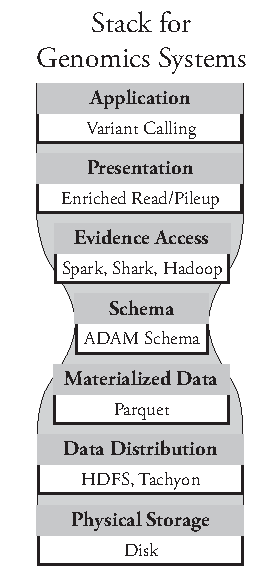
\includegraphics[width=0.25\linewidth]{stack-model.pdf}
\end{center}
\caption{A Stack Model for Scientific Computing}
\label{fig:stack-model}
\end{figure}

While the abstraction inversion used in genomics to accelerate common access patterns is undesirable
because it violates data independence, we also find that it sacrifices performance and
accuracy. The current Sequence/Binary Alignment and Map~(SAM/BAM~\cite{li09}) formats for storing
genomic alignments apply constraints about record ordering to enable specific computing patterns. Our
implementation~(described in~\S\ref{sec:genomics-pipeline}) identifies errors in two current genomics
processing stages that occur \emph{because} of the sorted access invariant. Our implementations of
these stages do not make use of sort order, and achieve higher performance \emph{while} eliminating
these errors.

Additionally, this thesis describes the variant discovery and genotyping algorithms implemented in
\texttt{avocado}. \texttt{avocado} introduces a new algorithm for local reassembly that eliminates the
expensive step of realigning reads to candidate haplotypes. Additionally, \texttt{avocado} introduces
a novel statistical model for genotyping that eliminates errors caused by statistical models that
optimistically assume the local independence of genomic loci.

All of the software~(source code and executables) described in this thesis are available free of charge
under the permissive Apache 2 open-source license. \texttt{ADAM} is available at
\url{https://www.github.com/bigdatagenomics/adam}, and \texttt{avocado} is available at
\url{https://www.github.com/bigdatagenomics/avocado}.

\section{Background}
\label{sec:background}

Our work is at the intersection of computational science, data management, and processing
systems. As such, our architectural approach is informed by recent trends in both areas. The design of
large scale data management has changed dramatically since the papers by Dean and
Ghemawat~\cite{dean04, dean08} that described Google's \texttt{MapReduce} system. Over a
similar timeframe, scientific fields have moved to take advantage of improvements in data acquisition
technologies. For example, since the Human Genome Project finished in 2001~\cite{lander01}, the price
of genomic sequencing has dropped by 10,000$\times$~\cite{nhgri}. This drop in cost has enabled the
capture of petabytes of sequence data, which has (in turn) enabled significant population genomics
experiments like the 1000 Genomes project~\cite{siva08} and The Cancer Genome Atlas~(TCGA,
\cite{weinstein13}). These changes are not unique to genomics; indeed, fields such as
neuroscience~\cite{cunningham14} and astronomy~\cite{lsst2008, turk11, sdss2000} are experiencing similar
changes.

Although there has been significant progress in the development of systems for processing large
datasets---the development of first generation MapReduce systems~\cite{dean04}, followed by
iterative MapReduce systems like Spark~\cite{zaharia10}, as well as parallel and columnar
DBMS~\cite{abadi06, lamb12}---the uptake of these systems in the scientific world has been slow.
Most implementations have either used MapReduce as an inspiration for API
design~\cite{mckenna10}, or have been limited systems that have used MapReduce to na\"{i}vely
parallelize existing toolkits~\cite{langmead09, schatz09}. These approaches are perilous for several
reasons:

\begin{itemize}
\item A strong criticism levied against the MapReduce model is that the API is insufficiently expressive
for describing complex tasks. As a consequence of this, tools like the GATK~\cite{mckenna10} that
adopt MapReduce as a programming model force significant restrictions on algorithm implementors. For
example, a GATK \texttt{walker}\footnote{The GATK provides \texttt{walker}s as an interface for
traversing regions of the genome.} is provided with a single view over the data~(a sorted iterator over a
specified region), and is allowed limited reduce functionality.
\item A major contribution of systems like MapReduce~\cite{dean08} and Spark~\cite{zaharia10,
zaharia12} is the ability to reliably distribute parallel tasks across a cluster in an automated fashion. While
the GATK uses MapReduce as a programming abstraction~(i.e., as an interface for writing
\texttt{walker}s), it does not use MapReduce as an execution strategy. To run tools like the GATK across
a cluster, organizations use workflow management systems for sharding and persisting intermediate
data, and managing failures and retries. This approach is not only an inefficient duplication of work, but it is also a
source of inefficiency during execution: the performance of iterative stages in the GATK is bottlenecked
by I/O performance.
\item The na\"{i}ve Hadoop-based implementations in Crossbow~\cite{langmead09} and
Cloudburst~\cite{schatz09} use scripts to run unmodified legacy tools on top of Hadoop. This approach does
achieve speedups, but does not attack any overhead. Several of the methods that they parallelize incur
high overhead due to duplicated loading of indices (for fast aligners, loading of large indices can be a
primary I/O bottleneck) and poor broadcasting of data.
\end{itemize}

Recent work by Diao et al~\cite{diao15} has looked at optimizations to MapReduce systems for
processing genomic data. They adapt strategies from the query optimization literature to reorder
computation to minimize data shuffling. While this approach does improve shuffle traffic, several
preprocessing stages cannot be transposed. For instance, reversing the order of indel realignment and
base quality score recalibration~(see~\S\ref{sec:genomics-pipeline}) will change the inferred quality
score distribution. Additionally, we believe that the shuffle traffic that Diao et al observe is an artifact
caused by the abstraction inversion discussed in~\S\ref{sec:introduction}. As we demonstrate
in~\S\ref{sec:genomics-pipeline}, these penalties can be eliminated by restructuring the pre-processing
algorithms.

One notable area where modern data management techniques have been leveraged by scientists is in
the data storage layer. Due to the storage costs of large genomic datasets, scientists have introduced the
CRAM format that uses columnar storage techniques and special compression algorithms to achieve a
30\% reduction in size over the original BAM format~\cite{fritz11}. While CRAM achieves high~($\gg 50\%$)
compression, it imposes restrictions on the ordering and structure of the data, and does not provide
support for predicates or projection. We perform a more comprehensive comparison against CRAM
in~\S\ref{sec:column-store-perf}.

One interesting trend of note is the development of databases specifically for scientific applications.
The exemplar is SciDB, which provides an array based storage model as well as efficient
linear algebra routines~\cite{brown10}. While arrays accelerate many linear algebra based routines, they
are not a universally great fit. For many genomics workloads, data is semistructured and may consist of
strings, boolean fields, and an array of tagged annotations. Other systems like the Genome Query
Language~\cite{kozanitis14} have extended SQL to provide efficient query semantics across genomic
coordinates. While GQL achieves performance improvements of up to 10$\times$ for certain algorithms,
SQL is not an attractive language for many scientific domains, which make heavy use of user designed
functions that may be cumbersome in SQL.

\section{Characteristics of Scientific Analysis Systems}
\label{sec:principles}

Most prior work on scientific computing has been focused on linear algebra and other problems that can
be structured as a matrix or network. However, in several of the emerging data-driven scientific
disciplines, data is less rigorously structured. As discussed
in~\S\ref{sec:background}, scientists have been developing ad hoc solutions to process this data. In this
section, we discuss the common characteristics of workloads in these emerging scientific areas. Given
these characteristics, we describe a way to decompose data processing and storage systems so that
we can efficiently implement important processing patterns while providing a wide range of data access
methods.

\subsection{Layering}
\label{sec:layering}

The processing patterns being applied to scientific data shift widely
as the data itself ages. Because of this change, we want to design a scientific data processing system that is
flexible enough to accommodate our different use cases. At the same time, we want to ensure that the
components in the system are well isolated so that we avoid bleeding functionality across the stack. If
we bleed functionality across layers in the stack, we make it more difficult to adapt our stack to different
applications. Additionally, as we discuss in~\S\ref{sec:genomics-pipeline}, improper separation of
concerns can actually lead to errors in our application.

These concerns are very similar to the factors that led to the development of the Open Systems
Interconnection~(OSI) model and Internet Protocol~(IP) stack for networking
services~\cite{zimmermann80}. The networking stack models were designed to allow the mixing and
matching of different protocols, all of which existed at different functional levels. The success of the
networking stack model can largely be attributed to the ``narrow waist'' of the stack, which simplified the
integration of a new protocol or technology by ensuring that the protocol only needed to implement a
single interface to be compatible with the rest of the stack.

Unlike conventional scientific systems that leverage custom data formats like BAM/SAM~\cite{li09},
or CRAM~\cite{fritz11}, we believe that the use of an explicit schema for data interchange is critical.
In our stack model shown in Figure~\ref{fig:stack-model}, the schema becomes the ``narrow waist''
of the stack. Most importantly, placing the schema as the narrow waist enforces a strict separation
between data storage/access and data processing. Additionally, this enables literate programming
techniques which can clarify the data model and access patterns. The seven layers of our stack model
are decomposed as follows, and are numbered in ascending order from bottom to top:

\begin{enumerate}
\item {\bf Physical Storage:} This layer coordinates data writes to physical media.
\item {\bf Data Distribution:} This layer manages access, replication, and distribution of the files that have
been written to storage media.
\item {\bf Materialized Data:} This layer encodes the patterns for how data is encoded and stored. This
layer determines I/O bandwidth and compression.
\item {\bf Data Schema:} This layer specifies the representation of data, and forms the narrow waist of
the stack that separates access from execution.
\item {\bf Evidence Access:} This layer provides us with primitives for processing data, and allows us to
transform data into different views and traversals.
\item {\bf Presentation:} This layer enhances the data schema with convenience methods for performing
common tasks and accessing common derived fields from a single element.
\item {\bf Application:} At this level, we can use our evidence access and presentation layers to compose
the algorithms to perform our desired analysis.
\end{enumerate}

A well defined software stack has several other significant advantages. By limiting application
interactions with layers lower than the presentation layer, application developers are given a clear and
consistent view of the data they are processing, and this view of the data is independent of whether the
data is local or distributed across a cluster or cloud. By separating the API from the data access layer,
we improve flexibility. With careful design in the data format and data access layers, we can seamlessly
support conventional whole file access patterns, while also allowing easy access to small slices of files.
By treating the compute substrate and storage as separate layers, we also drastically increase
the portability of the APIs that we implement.

As we discuss in more detail in~\S\ref{sec:genomics-pipeline}, current scientific systems bleed
functionality between stack layers. An exemplar is the SAM/BAM and CRAM formats, which expect data
to be sorted by genomic coordinate. This modifies the layout of data on disk~(level 3, Materialized Data)
and constrains how applications traverse datasets~(level 5, Evidence Access). Beyond
constraining applications, this leads to bugs in applications that are difficult to detect.\footnote{The
current best-practice implementations of the BQSR and Duplicate Marking algorithms both fail in certain
corner-case alignments. These errors are caused because of the limitation on traversing reads in sorted
order.} To resolve this conflict, we demonstrate several ways to efficiently implement conventional scientific
traversals in~\S\ref{sec:optimizations-scientific-processing}. These traversals are implemented in the
evidence access layer, and are independent of anything below the schema.

The idea of decomposing scientific applications into a stack model is not new; Bafna et al~\cite{bafna13}
made a similar suggestion in 2013. We borrow some vocabulary from Bafna et al, but our approach is
differentiated in several critical ways:

\begin{itemize}
\item Bafna et al consider the stack model specifically in the context of data management systems for
genomics; as a result, they bake current technologies and design patterns into the stack. In our opinion,
a stack design should serve to abstract layers from methodologies/implementations. If not, future
technology trends may obsolete a layer of the stack and render the stack irrelevant.
\item Bafna et al define a binary data format as the narrow waist in their stack, instead of a schema.
While these two seem interchangeable, they are not in practice. A schema is a higher level of abstraction
that encourages the use of literate programming techniques and allows for data serialization techniques to be
changed as long as the same schema is still provided.
\item Notably, Bafna et al use this stack model to motivate GQL~\cite{kozanitis14}. While a query system
should provide a way to process and transform data, Bafna et al instead move this system down to the
data materialization layer. We feel that this inverts the semantics that a user of the system would prefer
and makes the system less general.
\end{itemize}

Our stack enables us to serve the use cases we outline in~\S\ref{sec:workloads}. By using
Parquet as a storage format, we are able to process the data in many Hadoop-based systems. We
implement high performance batch and interactive processing with Spark, and can delegate to systems
like Impala and Spark-SQL for warehousing.

\subsection{Workloads}
\label{sec:workloads}

There are several common threads that unify the diverse set of applications that make up scientific
computing. When looking at the data that is used in different fields, several trends pop out:

\begin{enumerate}
\item Scientific data tends to be rigorously associated with coordinates in some domain. These coordinate
systems vary, but can include:
\begin{itemize}
\item Time~(e.g., fMRI data, particle simulations)
\item Chromosomal position~(e.g., genomic read alignments and variants)
\item Position in space~(imaging data, some sensor datasets)
\end{itemize}
\item For aggregated data, we frequently want to slice data into many different views. For example, for time
domain data aggregated from many sensors, scientists may want to perform analyses by slicing
across a single point in time, or by slicing across a single sensor. In genomics, we frequently aggregate data
across many people from a given population. Once we have done this first aggregation, we may want to then
slice the data by subsets of the population, or by regions of the genome~(e.g., specific genes of interest).
\end{enumerate}

There are two important consequences of the characteristics above. First, since data is attached to a
coordinate system, the coordinate system itself may impose logical processing patterns. For example, for
time domain data, we may frequently need to run functions that pass a sliding window across the dataset (e.g., for
convolution). Second, the slicing of aggregated data is frequently used to perform analyses across
subsets of a larger dataset. This is common if we want to study a specific phenomenon, like the role of a
gene in a disease~(a common analysis in the TCGA~\cite{weinstein13}), or the measured activity in a
single lobe of the brain while performing a task. Since the datasets we are processing are
large,\footnote{For example, the Acute Myeloid Leukemia subset of the TCGA alone is over 4 TB in size, and
is only one of 20 cancers in the TCGA.} it may be uneconomical to colocate data with processing nodes,
because of either the number of nodes that would need to be provisioned, or the amount of storage that would
need to be provisioned per node.

For scientific fields that process very large datasets, the exact processing techniques and algorithms vary
considerably, but common processing trends do exist:

\begin{enumerate}
\item There is increasing reliance on statistical methods. The \texttt{Thunder} pipeline makes heavy use
of the MLI/MLLib statistical libraries~\cite{freeman14, sparks13}, and tools like the GATK perform multiple
rounds of statistical refinement~\cite{depristo11}.
\item Data parallelism is very common. This varies across applications; in some applications (like
genomics), we may leverage the independence of sites across a coordinate system and process
individual coordinate regions in parallel. For other systems, we may have matrix calculations that can
be parallelized~\cite{sparks13}, or we may be able to run processing in parallel across samples or traces.
\end{enumerate}

Additionally, there are several different emerging use cases for scientific data processing and storage
systems. These different use cases largely correspond to different points in the lifecycle of the data:

\begin{itemize}
\item \textbf{Batch processing:} After the initial acquisition of raw sensor data~(e.g., raw DNA reads,
brain electrode traces, telescope images), we use a batch processing pipeline~(e.g., \texttt{Thunder} or
the GATK) to perform some dimensionality reduction/statistical summarization of the data. This is
generally used to extract notable features from the data, such as turning raw genomic reads into variant
alleles, or identifying areas of activity in neuroscience traces. These tasks are unlikely to have any
interactive component, and are likely to be long running compute jobs.
\item \textbf{Ad hoc exploration:} Once the batch processing has completed, there is often a need
for exploratory processing of the results. For example, when studying disease genetics, a geneticist may
use the variant/genotype statistics to identify genomic sites with statistically significant links to the
disease phenotype. Data exploration tasks have a significant user facing/interactive nature, and are
generally performed by scientists who may be programming laypeople.
\item \textbf{Data warehousing:} In large scientific projects, it is common to make data available to the
members of the scientific community through some form of warehouse service~(e.g., the Cancer
Genomics Hub, CGHub, for the TCGA). As is the case for all data warehousing, this implies that queries
must be made reasonably efficient, even though the data is expected to be cold. To reduce the cost of
storing data, we may prioritize compression here; this has led to the creation of compressed storage
formats like CRAM~\cite{fritz11}.
\end{itemize}

In this paper, we design a system that can achieve all of the above goals. The genomics and
astronomy pipelines we demonstrate achieve improvements in batch processing performance, and
allow for interactive/exploratory analysis through both Scala and Python. Through the layering principles
we lay out in the next section and the performance optimizations we introduce
in~\S\ref{sec:loading-remote-data}, we make our system useful for warehousing scientific data.

\section{Related Work}
\label{sec:related-work}

Similar to what we propose, the \texttt{Thunder} system was developed as a novel MapReduce-based system for
processing terabytes of neuroscience imaging data~\cite{freeman14}. \texttt{Thunder} performs a largely statistical
workload, and the significant tasks in terms of execution time are clustering and regression. The system is
constructed using Spark and Python and is designed to process datasets larger than 4 TB, and leverages
significant functionality from the MLI/MLLib libraries~\cite{sparks13}. Similar to our system, they are able to use
Spark's in-memory caching to amortize load time across several pipeline stages. Additionally, they use Spark's
filtering primitives to allow scientists to cut problems into subproblems. This is a common trend across scientific
analyses, and is one of the reasons that we advocate for the use of a columnar store with efficient predicate
pushdown. \texttt{Thunder} is an example pipeline that demonstrates the power of using horizontally scalable
systems to enable novel scientific analyses.

\chapter{Genomic Data Storage and Preprocessing Using \texttt{ADAM}}

To validate our architectural choices, we have implemented pipelines for processing short read genomic
data and astronomy image processing. Both of these pipelines are implemented using
Spark~\cite{zaharia10}, Avro~\cite{avro}, and Parquet~\cite{parquet}. We have chosen these two
applications as they fit in different areas in the design space. Specifically, the genomics pipeline makes
heavy use of statistical processing techniques over semistructured data, while the astronomy application
has a traditional matrix structure.

Corresponding to the stack model that was introduced in Figure~\ref{fig:stack-model}, we use the
following technologies to implement both of our applications:

\begin{itemize}
\item \textbf{Physical Storage:} We have designed our system to run on top of local or distributed
drives, as well as block stores.
\item \textbf{Data Distribution:} Our system is designed to operate on top of the Hadoop Distributed File
System~(HDFS), or to perform it's own data distribution over HTTP or by reaching out to an Amazon
S3 bucket. We describe these optimizations in~\S\ref{sec:loading-remote-data}.
\item \textbf{Materialized Data:} We store data using the open source Parquet columnar store.
\item \textbf{Schema:} We manage our schemas~(and data serialization) via the Avro serialization
framework~\cite{avro}. Our schemas are described in Appendix~\ref{sec:schema}.
\item \textbf{Evidence Access:} We use Spark's Resilient Distributed Dataset~(RDD, \cite{zaharia12})
abstraction to provide parallel processing over the data. We enhance this with the join patterns we
describe in~\S\ref{sec:coordinate-system-joins}.
\item \textbf{Presentation:} In our genomics application, we provide several rich datatypes that implicitly
wrap our schemas to provide convenience methods for metadata access. This is not as crucial in the
astronomy application.
\end{itemize}

In the remainder of this section, we describe the two applications that we have implemented, and the
optimizations we have made to improve the horizontal scalability of these algorithms.

\section{Pipeline Structure}
\label{sec:genomics-pipeline}

Contemporary genomics has been revolutionized by ``next generation'' sequencing
technologies~(NGS), which have driven a precipitous drop in the cost of running genomic
assays~\cite{nhgri}. Although there are a variety of sequencing technologies in use, the majority of
sequence data comes from the Illumina sequencing platform, which uses a ``sequencing-by-synthesis''
technique to generate short read data~\cite{metzker09}. Short read refers to 
sequencing run will generate many reads that are between 50 and 250 bases in length. In addition to
adjusting the length of the reads, we can control the amount of the data that is generated by
changing the amount of the genome that we sequence, or the amount of redundant sequencing that
we perform~(the average number of reads that covers each base, or \emph{coverage}). A single
human genome sequenced at 60$\times$ coverage will produce approximately 1.4 billion reads,
which is approximately 600 GB of raw data, or 225 GB of compressed data. For each read, we also
are provided \emph{quality scores}, which represent the likelihood that the base at a given position
was observed.

One of the most common genomic analyses is \emph{variant calling}, which is a statistical process to
infer the sites at that a single individual varies from the reference genome.\footnote{The
reference genome represents the ``average'' genome for a species. The Human Genome
Project~\cite{lander01} assembled the first human reference genome.} To call variants, we perform the
following steps:

\begin{enumerate}
\item \textbf{Alignment:} For each read, we find the position in the genome that the read is most likely to
have come from. As an exact search is too expensive, there has been an extensive amount of research
that has focused on indexing strategies for improving alignment performance~\cite{li10, li11,
zaharia11}. This process is parallel per sequenced read.
\item \textbf{Pre-processing:} After reads have been aligned to the genome, we perform several
preprocessing steps to eliminate systemic errors in the reads. This may involve recalibrating the
observed quality scores for the bases, or locally optimizing the read alignments. We will present a
description of several of these algorithms in~\S\ref{sec:genomics-pipeline}; for a more detailed
discussion, we refer readers to DePristo et al~\cite{depristo11}.
\item \textbf{Variant calling:} Variant calling is a statistical process that uses the read alignments
and the observed quality scores to compute whether a given sample matches or diverges
from the reference genome. This process is typically parallel per position or region in the genome.
\item \textbf{Filtration:} After variants have been called, we want to filter out false positive variant calls.
We may perform queries to look for variants with borderline likelihoods, or we may look for clusters of
variants, which may indicate that a local error has occurred. This process may be parallel per position,
may involve complex traversals of the genomic coordinate space, or may require us to fit a statistical
model to all or part of the dataset. While we do not present work on variant filtration in this paper, variant
filtration has motivated the coordinate space joins presented in~\S\ref{sec:coordinate-system-joins}.
\end{enumerate}

This process is very expensive in time to run; the current best practice pipeline uses the BWA tool~\cite{li10} for
alignment and the GATK~\cite{depristo11, mckenna10} for pre-processing, variant calling, and filtration.
Current benchmark suites have measured this pipeline as taking between 90 and 130 hours to run
end-to-end~\cite{talwalkar14}. Recent projects have achieved 5--$10\times$ improvements in alignment
and variant calling performance~\cite{rimmer14, zaharia11}, which makes the pre-processing stages
the performance bottleneck. Our experimental results have corroborated this, as the four pre-processing stages
take over 110 hours to run on a clinical quality human genome when run on an Amazon EC2 \texttt{cr1.8xlarge}
machine. 

For current implementations of these read processing steps, performance is limited by disk
bandwidth~\cite{diao15}. This bottleneck exists because the operations read in a SAM/BAM file, perform
a small amount of processing, and write the data to disk as a new SAM/BAM file. We achieve a
performance bump by performing our processing iteratively in memory. The four read processing stages
can then be chained together, eliminating three long writes to disk and an additional three long reads
from disk. Additionally, by rethinking the design of our algorithms, we are able to reduce overhead in
several other ways:

\begin{enumerate}
\item Current algorithms require the reference genome to be present on all nodes. This assembly is then used to
look up the reference sequence that overlaps all reads. The reference genome is several gigabytes in
size, and performing a lookup in the reference genome can be costly due to its size. Instead, we leverage
the \texttt{mismatchingPositions} field in our schema to embed information about the reference in each read. This
optimization allows us to avoid broadcasting the reference, and provides O(1) lookup.
\item Shared-memory genomics applications tend to be impacted significantly by false sharing of data
structures~\cite{zaharia11}. Instead of having data structures that are modified in parallel, we
restructure our algorithms so that we only touch data structures from a single thread, and then merge
structures in a reduce phase. The elimination of sharing improves the performance of covariate calculation during
BQSR and the target generation phase of local realignment.
\item In a na\"{i}ve implementation, the local realignment and duplicate marking tasks can suffer from
stragglers. The stragglers occur due to a large amount of reads that either do not associate to a realignment
target, or that are unaligned. We pay special attention to these cases by manually randomizing the
partitioning for these reads. This resolves load imbalance and mitigates stragglers.
\item For the Flagstat command, we are able to project a limited subset of fields. Flagstat touches fewer
than 10 fields, which account for less than 10\% of space on disk. We discuss the performance
implications of this further in~\S\ref{sec:column-store-perf}.
\end{enumerate}

These techniques allow us to achieve a $>50\times$ performance improvement over current tools, and
scalability beyond 128 machines. We perform a detailed performance review
in~\S\ref{sec:genomics-performance}.

\section{Read Preprocessing Algorithms}
We have focused on implementing the four most-commonly used pre-processing stages, as well as
\texttt{flagstat}, a command that is used at the end of pre-processing for validating the quality of an
aligned/pre-processed sample. In the remainder of this section, we describe the stages that we have implemented,
and the techniques we have used to improve performance and accuracy.

\begin{enumerate}
\item \textbf{Sorting:} This phase sorts all reads by the position of the start of their alignment. The implementation
of this algorithm is trivial, as Spark provides a sort primitive~\cite{zaharia10}; we solely need to define an
ordering for genomic coordinates, which is well defined.\footnote{In practice, an explicit sort is unnecessary when
using the rest of our MapReduce-based pipeline. We have included sort to enable the use of legacy tools that
require sorted input.}
\item \textbf{Duplicate Removal:} During the process of preparing DNA for sequencing, reads are duplicated by
errors during the sample preparation and polymerase chain reaction stages. Detection of duplicate reads
requires matching all reads by their position and orientation after read alignment. Reads with identical position
and orientation are assumed to be duplicates. When a group of duplicate reads is found, each read is scored,
and all but the highest quality read are marked as duplicates.

We have validated our duplicate removal code against Picard~\cite{picard}, which is used by the GATK
for Marking Duplicates. Our implementation is fully concordant with the Picard/GATK duplicate removal
engine, except we are able to perform duplicate marking for chimeric read pairs.\footnote{In a chimeric read pair,
the two reads in the read pairs align to different chromosomes; see Li et al~\cite{li10}.}
Specifically, because Picard's traversal engine is restricted to processing linearly sorted alignments,
Picard mishandles these alignments. Since our engine is not constrained by the underlying layout of data
on disk, we are able to properly handle chimeric read pairs.
\item \textbf{Local Realignment:} In local realignment, we correct areas where variant alleles cause reads to be
locally misaligned from the reference genome.\footnote{This is typically caused by the presence of
insertion/deletion (INDEL) variants; see DePristo et al~\cite{depristo11}.} In this algorithm, we first identify regions
as targets for realignment. In the GATK, this is done by traversing sorted read alignments. In our implementation,
we fold over partitions where we generate targets, and then we merge the tree of targets. This process allows us
to eliminate the data shuffle needed to achieve the sorted ordering. As part of this fold, we must
compute the convex hull of overlapping regions in parallel. We discuss this in more detail in
Appendix~\ref{sec:convex-hull}.

After we have generated the targets, we associate reads to the overlapping target, if one exists. After
associating reads to realignment targets, we run a heuristic realignment algorithm that works by minimizing
the quality-score weighted number of bases that mismatch against the reference.
\item \textbf{Base Quality Score Recalibration~(BQSR):} During the sequencing process, systemic errors occur
that lead to the incorrect assignment of base quality scores. In this step, we label each base that we have
sequenced with an \emph{error covariate}. For each covariate, we count the total number of bases that we saw,
as well as the total number of bases within the covariate that do not match the reference genome. From this data, 
we apply a correction by estimating the error probability for each set of covariates under a beta-binomial model
with uniform prior:

\begin{equation}
\label{eqn:bqsrerr}
\mathbf{E}(P_{err}|{cov}) = \frac{\texttt{\#errors}(cov) + 1}{\texttt{\#observations}(cov) + 2}
\end{equation}

We have validated the concordance of our BQSR implementation against the GATK. Across both tools, only 5000
of the $\sim$180B bases~($<0.0001\%$) in the high-coverage NA12878 genome dataset differ. After investigating
this discrepancy, we have determined that this is due to an error in the GATK, where paired-end reads are
mishandled if the two reads in the pair overlap.
\end{enumerate}

\subsection{BQSR Implementation}
\label{sec:bqsr-implementation}

Base Quality Score Recalibration is an important early data-normalization step in the bioinformatics pipeline, and after alignment
it is the next most costliest step. Since quality score recalibration can vastly improve the accuracy of variant calls~---~particularly for
pileup-based callers like the UnifiedGenotyper or Samtools mpileup. Because of this, it is likely to remain a part of bioinformatics pipelines.

BQSR is also an interesting algorithm in that it doesn't neatly fit into the framework of map reduce (the design philosophy of the GATK).
Instead it is an embarrassingly parallelizable aggregate. The ADAM implementation is:

\begin{lstlisting}
def computeTable(rdd: Records, dbsnp: Mask) :
  RecalTable = {
  
  rdd.aggregate(new RecalTable)(
    (table, read) => { table + read },
    (table, table) => { table ++ table })
}
\end{lstlisting}

The ADAM implementation of BQSR utilizes the MD field to identify bases in the read that mismatch the reference. This enables
base quality score recalibration to be entirely reference-free, avoiding the need to have a central Fasta store for the human
reference. However, dbSNP is still needed to mask out positions that are polymorphic (otherwise errors due to real variation will
severely bias the error rate estimates).

\subsection{Indel Realignment Implementation}
\label{sec:indel-realignment-implementation}

Indel realignment is implemented as a two step process. In the first step, we identify regions that have evidence of an insertion or
deletion. After these regions are identified, we generate candidate haplotypes, and realign reads to minimize the overall quantity
of mismatches in the region. The quality of mismatches near an indel serves as a good proxy for the local quality of an alignment.
This is due to the nature of indel alignment errors: when an indel is misaligned, this causes a temporary shift in the read sequence
against the reference sequence. This shift manifests as a run of several bases with mismatches due to their incorrect alignment.

\subsubsection{Realignment Target Identification}
\label{sec:realignment-target-identification}

Realignment target identification is done by converting our reads into reference oriented ``rods''\footnote{Also known as pileups: a
group of bases that are all aligned to a specific locus on the reference.}. At each locus where there is evidence of an insertion or a
deletion, we create a \emph{target} marker. We also create a target if there is evidence of a mismatch. These targets contain the indel
range or mismatch positions on the reference, and the range on the reference covered by reads that overlap these sites.

After an initial set of targets are placed, we merge targets together. This is necessary, as during the read realignment process, all
reads can only be realigned once. This necessitates that all reads are members of either one or zero realignment targets. Practically,
this means that over the set of all realignment targets, no two targets overlap.

The core of our target identification algorithm can be found below.

\begin{lstlisting}
def findTargets (reads: RDD[ADAMRecord]):
    TreeSet[IndelRealignmentTarget] = {

  // convert reads to rods
  val processor = new Read2PileupProcessor
  val rods: RDD[Seq[ADAMPileup]] = reads.flatMap(
      processor.readToPileups(_))
    .groupBy(_.getPosition).map(_._2)

  // map and merge targets
  val targetSet = rods.map(
      IndelRealignmentTarget(_))
    .filter(!_.isEmpty)
    .keyBy(_.getReadRange.start)
    .sortByKey()
    .map(new TreeSet()(TargetOrdering) + _._2)
    .fold(new TreeSet()(TargetOrdering))(
      joinTargets)

  targetSet
}
\end{lstlisting}

To generate the initial unmerged set of targets, we rely on the ADAM toolkit's pileup generation utilities~(see~\-S\ref{sec:reference-oriented-storage}).
We generate realignment targets for all pileups, even if they do not have indel or mismatch evidence. We eliminate pileups that do not contain indels
or mismatches with a filtering stage that eliminates empty targets. To merge overlapping targets, we map all of the targets into a sorted set. This set
is implemented using Red-Black trees. This allows for efficient merges, which are implemented with the tail-call recursive \emph{joinTargets} function:

\begin{lstlisting}
@tailrec def joinTargets (                                                                                                                                                               
  first: TreeSet[IndelRealignmentTarget],                                                                                                                                                                
  second: TreeSet[IndelRealignmentTarget]):
    TreeSet[IndelRealignmentTarget] = {

  if (!TargetOrdering.overlap(first.last,
      second.head)) {
    first.union(second)
  } else {
    joinTargets (first - first.last +
      first.last.merge(second.head),
      second - second.head)
  }
}
\end{lstlisting}

As we are performing a fold on an RDD which is sorted by the starting position of the target on the reference sequence, we know a priori that the elements
in the ``first'' set will always be ordered earlier relative to the elements in the ``second'' set. However, there can still be overlap between the two sets, as this
ordering does not account for the end positions of the targets. If there is overlap between the last target in the ``first'' set and the first target in the ``second''
set, we merge these two elements, and try to merge the two sets again.

\subsubsection{Candidate Generation and Realignment}
\label{sec:candidate-generation-realignment}

Candidate generation is a several step process:

\begin{enumerate}
\item Realignment targets must ``collect'' the reads that they contain.
\item For each realignment group, we must generate a new set of candidate haplotype alignments.
\item Then, these candidate alignments must be tested and compared to the current reference haplotype.
\item If a candidate haplotype is sufficiently better than the reference, reads are realigned.
\end{enumerate}

The mapping of reads to realignment targets is done through a tail recursive function that performs a binary search across the sorted set of indel alignment targets:

\begin{lstlisting}
@tailrec def mapToTarget (read: ADAMRecord,                                                                                                                                                        
  targets: TreeSet[IndelRealignmentTarget]):
    IndelRealignmentTarget = {

  if (targets.size == 1) {
    if (TargetOrdering.equals (targets.head, read)) {
      targets.head
    } else {
      IndelRealignmentTarget.emptyTarget
    }
  } else {
    val (head, tail) = targets.splitAt(
      targets.size / 2)
    val reducedSet = if (TargetOrdering.lt(
        tail.head, read)) {
      head
    } else {
      tail
    }
    mapToTarget (read, reducedSet)
  }
}
\end{lstlisting}

This function is applied as a groupBy against all reads. This means that the function is mapped to the RDD that contains all reads. A new RDD is generated where all
reads that returned the same indel realignment target are grouped together into a list.

Once all reads are grouped, we identify new candidate alignments. However, before we do this, we left align all indels. For many reads that show evidence of a single
indel, this can eliminate mismatches that occur after the indel. This involves shifting the indel location to the ``left''\footnote{To a lower position against the reference
sequence.} by the length of the indel. After this, if the read still shows mismatches, we generate a new consensus alignment. This is done with the
\emph{generateAlternateConsensus} function, which distills the indel evidence out from the read.

\begin{lstlisting}
def generateAlternateConsensus (sequence: String,
  start: Long, cigar: Cigar): Option[Consensus] = {
  var readPos = 0
  var referencePos = start

  if (cigar.getCigarElements.filter(elem =>
        elem.getOperator == CigarOperator.I ||
        elem.getOperator == CigarOperator.D
      ).length == 1) {
    cigar.getCigarElements.foreach(cigarElement =>
      { cigarElement.getOperator match {
        case CigarOperator.I => return Some(
          new Consensus(sequence.substring(readPos,
            readPos + cigarElement.getLength),
            referencePos to referencePos))
        case CigarOperator.D => return Some(
          new Consensus("",
          referencePos until (referencePos +
            cigarElement.getLength)))
        case _ => {
          if (cigarElement.getOperator
                .consumesReadBases &&
              cigarElement.getOperator
                .consumesReferenceBases
              ) {
            readPos += cigarElement.getLength
            referencePos += cigarElement.getLength
          } else {
            return None
          }
        }
      }
    })
    None
  } else {
    None
  }
}
\end{lstlisting}

From these consensuses, we generate new haplotypes by inserting the indel consensus into the reference sequence. The quality of each haplotype is measured
by sliding each read across the new haplotype, using \emph{mismatch quality}. Mismatch quality is defined for a given alignment by the sum of the quality scores
of all bases that mismatch against the current alignment. While sliding each read across the new haplotype, we aggregate the mismatch quality scores. We take
the minimum of all of these scores and the mismatch quality of the original alignment. This sweep is performed using the \emph{sweepReadOverReferenceForQuality}
function:

\begin{lstlisting}
def sweepReadOverReferenceForQuality (
    read: String,reference: String,
    qualities: Seq[Int]): (Int, Int) = {
  var qualityScores = List[(Int, Int)]()

  for (i <- 0 until (reference.length -
      read.length)) {
    qualityScores = (
      sumMismatchQualityIgnoreCigar(
        read,
        reference.substring(i, i + read.length),
          qualities),
        i) :: qualityScores
  }

  qualityScores.reduce ((p1: (Int, Int),
      p2: (Int, Int)) => {
    if (p1._1 < p2._1) {
      p1
    } else {
      p2
    }
  })
}
\end{lstlisting}

If the consensus with the lowest mismatch quality score has a log-odds ratio~(LOD) that is greater than $5.0$ with respect to the reference, we realign the reads.
This is done by recomputing the cigar and MDTag for each new alignment. Realigned reads have their mapping quality score increased by 10 in the Phred scale.

\subsection{Duplicate Marking Implementation}
\label{sec:duplicate-marking-implementation}

The following ADAM code, reformatted for this report, expresses the algorithm succinctly in 42 lines of Scala code.

\begin{lstlisting}
for (((leftPos, library), readsByLeftPos) <- 
    rdd.adamSingleReadBuckets()
       .keyBy(ReferencePositionPair(_))
       .groupBy(leftPositionAndLibrary);

buckets <- {

leftPos match {
 // These are all unmapped reads. 
 // There is no way to determine if
 // they are duplicates
 case None =>
    markReads(readsByLeftPos.unzip._2,
      areDups = false)
 // These reads have their left position mapped
 case Some(leftPosWithOrientation) =>
   // Group the reads by their right position
   val readsByRightPos = readsByLeftPos.groupBy(
     rightPosition)
   // Find any reads with no right position
   val fragments = readsByRightPos.get(None)
   // Check if we have any pairs
   // (reads with a right position)
   val hasPairs = readsByRightPos.keys
     .exists(_.isDefined)
   if (hasPairs) {
     // Since we have pairs,
     // mark all fragments as duplicates
     val processedFrags = if (fragments.isDefined
     ) {
       markReads(fragments.get.unzip._2,
         areDups = true)
     } else {
       Seq.empty
     }
     val processedPairs = 
         for (buckets <- (readsByRightPos - None)
           .values;
             processedPair <- 
                scoreAndMarkReads(buckets.unzip._2)) 
        yield processedPair
     processedPairs ++ processedFrags
   } else if (fragments.isDefined) {
     // No pairs. Score the fragments.
     scoreAndMarkReads(fragments.get.unzip._2)
   } else {
     Seq.empty
   }
};
read <- buckets.allReads) yield read
\end{lstlisting}

For lines 1-4, all reads with the same record group name and read name are collected 
into buckets. These buckets contain the read and optional mate or secondary alignments.
Each read bucket is then keyed by 5 $'$ position and orientation and grouped together by
left (lowest coordinate) position, orientation and library name.

For lines 8-41, we processed each read bucket with a common left 5$'$ position. Unmapped
reads are never marked duplicate as their position is not known. Mapped reads with a common
left position are separated into paired reads and fragments. Fragments, in this context,
are reads that have no mate or should have a mate but it doesn't exist.

If there are pairs in a group, all fragments are marked duplicates and the paired reads are grouped
by their right 5$'$ position. All paired reads that have a common right and left 5$'$
position are scored and all but the highest scoring read is marked a duplicate.

If there are no pairs in a group, all fragments are scored and all but the highest scoring fragment
are marked duplicates.

\chapter{Variant Calling via Reassembly Using \texttt{avocado}}

\section{Reference Threaded \emph{de Bruijn} Graphs}

The local assembler in \texttt{avocado} is a de bruijn graph based assembler. The assembler creates
a ``reference threaded'' assembly. In this approach, we label $k$-mers that appear in the
reference genome with their reference position. The advantage of this approach is that we can
determine whether a $k$-mer in the graph can be mapped to the reference genome or if it
represents a divergence from the reference (an alternate allele). Additionally, for bubbles
off of reference arcs, we can identify the exact allele represented by the bubble without
needing to enumerate haplotypes which we then align against the reference sequence. This
approach has the following benefits:

\begin{itemize}
\item For a region that contains $n$ variants, we only need to evaluate $n$ variant arcs, as
opposed to $n^2$ variant haplotypes.
\item We can emit statistics for computing genotype likelihoods directly from the de bruijn
graph. This is more efficient than emitting all haplotypes, scoring haplotype pairs, and
then realigning reads to the top scoring haplotype pair.
\end{itemize}

\subsection{Formulation}

First, we start with the traditional formulation of a \emph{de bruijn} graph for sequence assembly:

\begin{itemize}
\item Each $k$-mer $s$ represents a $k$-length string, with a $k - 1$ length prefix given by
$\text{prefix}(s)$ and a length 1 suffix given by $\text{suffix}(s)$.
\item We place a directed edge ($\rightarrow$) from $k$-mer $s_1$ to $k$-mer $s_2$ if
$\text{prefix}(s_1)^{\{1, k - 2\}} + \text{suffix}(s_1) = \text{prefix}(s_2)$.
\end{itemize}

Additionally, we add the following:

\begin{itemize}
\item There is a set $\mathcal{R}$ which contains all of the $k$-mers that are in the reference
genome that covers a certain region.
\item If $k$-mer $s \in \mathcal{R}$, then the output of function $\text{refPos}(s)$ is defined.
This function provides us with the integer position of $s$ in the reference genome.
\item For two $k$-mers $s_1, s_2 \in \mathcal{R}$, we can define a distance function
$\text{distance}(s_1, s_2) = | \text{refPos}(s_1) - \text{refPos}(s_2) |$.
\end{itemize}

As stated above, this condition assumes that there is a 1-dimensional reference (e.g., a single
assembled reference). In reality, genomic assemblies provide a 2-dimensional space, where the
second dimension is defined by the chromosome that we are on. In practice, we will reassemble
reads from a region which is restricted to a single chromosome.

To discover alternate alleles from this graph without performing a search for all haplotypes,
we need to address the $k$-mers that are not in $\mathcal{R}$. These can be processed with
path-based methods. First, let us classify paths into two types:

\begin{itemize}
\item \textbf{Spurs:} A spur is a set $S$ of $n$ $k$-mers $\{s_1, \dots, s_n\}$ where either $s_1$ or
$s_n \in \mathcal{R}$ and all other $k$-mers are $\not\in \mathcal{R}$, and where
$s_i \rightarrow s_{i + 1} \forall i \in \{1, \dots, n - 1\}$. If $s_1 \in \mathcal{R}$,
then $s_n$ must not have a successor. Alternatively, if $s_n \in \mathcal{R}$, than $s_1$ is
required to not have a predecessor.
\item \textbf{Bubbles:} A bubble is a set $S$ of $n$ $k$-mers $\{s_1, \dots, s_n\}$ where both
$s_1$ and $s_n \in \mathcal{R}$ and all other $k$-mers are $\not\in \mathcal{R}$, and where
$s_i \rightarrow s_{i + 1} \forall i \in \{1, \dots, n - 1\}$.
\end{itemize}

Currently, we do not process spurs. Spurs typically result from sequencing errors near the
start or end of a read. Additionally, given a spur, we cannot put a constraint on what sort of
edit it may be from the reference.

However, it is easy to define constraints for bubbles so that we can determine what variant
has been seen at that site. For many variants, we can even canonically determine the variant.
First, let us make three definitions:

\begin{itemize}
\item The \emph{bubble length} is the number of non-reference $k$-mers that appear in the bubble.
\item The \emph{gap length} is the distance between $s_1$ and $s_n$ in the reference genome. Formally,
$l_{\text{gap}} = \text{distance}(s_1, s_n)$.
\item The \emph{allele length} is the absolute difference between the bubble length and the gap length.
\end{itemize}

With these definitions, we can define the allelic composition of bubbles as follows:

\begin{itemize}
\item A bubble contains a single/multiple nucleotide variant (S/MNV) if $l_{\text{allele}} = 0$.
\item A bubble contains a canonical insert if $l_{\text{bubble}} = l_{\text{gap}} + l_{\text{allele}}$.
\item A bubble contains a canonical deletion if $l_{\text{bubble}} < k$, where $k$ is the $k$-mer size,
and $\text{distance}(s_1, s_n) > 0$.
\item If a bubble does not meet any of the above constraints, it is a non-canonical indel.
\end{itemize}

We discuss how to process these alleles in \S\ref{sec:reassembly-implementation}. It
is also worth noting that this approach can be used for detecting structural variants. A simple
extension involves jointly processing multiple reference regions (e.g., $\mathcal{R}_1$ and
$\mathcal{R}_2$). If $s_1$ and $s_n$ are members of different reference sets, then this bubble
identifies a possible structural variant breakpoint. While this section has just provided intuition about the
canonical representation of alleles from a de bruijn graph, we provide full proofs
in~\S\ref{sec:canonical-proofs} at the end of this chapter.

\subsection{Reassembly Implementation}
\label{sec:reassembly-implementation}

Reassembly is performed as a two step process. In the first step, we build a reference threaded
de bruijn graph using the sequence of reference region $\mathcal{R}$ and the reads from sample $n$.
Once we have built a reference threaded de bruijn graph, we then elaborate the graph and identify
the allelic content of all bubbles.

\subsubsection{Graph Construction}
\label{sec:graph-construction}

A reference threaded de bruijn graph is constructed per sample. We start by extracting the
reference $k$-mers. This algorithm---\texttt{addReferenceKmers}---is tail recursive.

\begin{algorithm}
\caption{Incorporate Reference \emph{k}-mers: \texttt{addReferenceKmers(iter, pos, lastKmer, kmerMap)}}
\label{alg:build-reference-kmers}
\begin{algorithmic}
\STATE $iter \leftarrow$ iterator across $k$-mer strings from the reference
\STATE $pos \leftarrow$ current reference position
\STATE $lastKmer \leftarrow$ the last $k$-mer seen
\STATE $kmerMap \leftarrow$ a map from $k$-mer strings $\rightarrow$ objects
\IF{$iter \ne \emptyset$}
\STATE $ks \leftarrow iter$.next
\IF{$lastKmer \ne \emptyset$}
\STATE $newKmer \leftarrow $ \texttt{Kmer(} $ks$, $pos$, $predecessors = \{lastKmer\}$\texttt{)}
\STATE $lastKmer$.$successors \leftarrow lastKmer$.$successors + newKmer$
\ELSE
\STATE $newKmer \leftarrow $ \texttt{Kmer(} $ks$, $pos$\texttt{)}
\ENDIF
\STATE $newPos \leftarrow pos + 1$
\STATE $kmerMap \leftarrow kmerMap + (ks, newKmer)$
\STATE \texttt{addReferenceKmers(} $iter$, $newPos$, $newKmer$, $kmerMap$\texttt{)}
\ENDIF
\end{algorithmic}
\end{algorithm}

We use a similar algorithm for processing the $k$-mers from the read dataset. However, this
algorithm filters out $k$-mers that contain \texttt{N}s, checks to see whether the $k$-mer
sequence has been seen before, and also stores information about the mapping quality, base
quality, and read strand.

\subsubsection{Graph Elaboration}
\label{sec:graph-elaboration}

To elaborate the graph (the \texttt{toObservations} class method of a \texttt{KmerGraph}), we rely on a
tail-recursive state machine that pushes state onto a stack at branch points. Our machine
has the following states:

\begin{itemize}
\item \texttt{R}, \texttt{Reference}: We are on a run of $k$-mers that are mapped to a position in $\mathcal{R}$.
\item \texttt{A}, \texttt{Allele}: We are on a run of $k$-mers that have diverged off of the reference. We have a
divergence start point, but have not connected back to the reference yet. This could be either
a bubble or a spur. 
\item \texttt{C}, \texttt{ClosedAllele}: We were on a run of $k$-mers that had diverged off of the reference, but
have just reconnected back to the reference and now know the start and end positions of the bubble,
as well as the alleleic content of the bubble.
\end{itemize}

The following state transitions are allowed:

\begin{itemize}
\item \texttt{R} $\rightarrow$ \texttt{R}: We are continuing along a reference run.
\item \texttt{R} $\rightarrow$ \texttt{A}: We were at a reference mapped $k$-mer, and have seen a branch to a
non-reference $k$-mer.
\item \texttt{A} $\rightarrow$ \texttt{A}: We are continuing along a non-reference run.
\item \texttt{A} $\rightarrow$ \texttt{C}: We were on a non-reference run, and have just connected back to a
reference $k$-mer.
\item \texttt{C} $\rightarrow$ \texttt{R}: We have just closed out an allele, and are back at a reference position.
\end{itemize}

We initialize the state machine to `R` with the first $k$-mer from $\mathcal{R}$. Per $k$-mer,
we evaluate the state transition per successor $k$-mer. If the successor set contains a single
$k$-mer, we continue to that state. If the successor set contains multiple $k$-mers, we choose
a successor state to transition to, and push the branch context of all other successor states
onto our stack. If the successor set is empty, we pop a branch context off of the stack, and
switch to that context. We stop once we reach a $k$-mer whose successor set is empty, and our
branch context stack is empty.

The implementation of the \texttt{R} and \texttt{A} states are trivial and largely amount to bookkeeping.
The \texttt{C} state though, is more complex. First, let us discuss how to canonicalize the canonical
alleles:

\begin{itemize}
\item For a canonical S/MNV bubble, the SNV sites can be determined by calculating the Hamming distance
of the bubble sequence versus the reference sequence. Evidence for SNVs exist at any site
where an edit is made.
\item For a canonical insert, sequence is inserted $k - 1$ bases from the bubble start. There will be
$l_{\text{allele}}$ bases inserted. We can derive the inserted bases by computing the bubble
sequence and trimming the first $k - 1$ bases.
\item For a canonical deletion, we guarantee that the bubble sequence is derived from the start and
end of the reference sequences that the bubble overlaps. To canonicalize this, we can perform
a greedy match of the bubble sequence, where we match bases to the front of the deletion until
we see a mismatch, and then align all remaining bases to the end of the deletion.
\end{itemize}

For a complex variant, we take the bubble sequence and align it against the reference sequence
from the bubble gap using a pairwise HMM~\cite{durbin98}. From the HMM alignment, we
emit observations according to the observed alignment states. The HMM uses an infinite padding
penalty to ensure that the ends of the sequences are matched.

\section{Statistical Models for Genotyping}
\label{sec:statistical-genotyping}

Given a set of observed alleles and reads spanning these alleles, we can put together a graph. Each
allele is given a node. We connect two nodes with an edge if and only if a read is observed to cover both
nodes. In Figure~\ref{fig:alleles}, we present a sequence where the reference is
\texttt{ACCCTATCGCTCACA}. Evidence of a \texttt{C} $\rightarrow$ \texttt{G} single nucleotide
polymorphism~(SNP) is present at position 3, and evidence of a deletion of bases 8--9 (\texttt{GC}) is
present.

\begin{figure}[h]
\begin{center}
\includegraphics[width=0.4\linewidth]{graphs/alleles.pdf}
\end{center}
\caption{Allele Graph}
\label{fig:alleles}
\end{figure}

Between two nodes, we can define a conditional probability $P(x = X | y = Y)$, which is the probability that
node $x$ has copy number $X$ and node $y$ has copy number $Y$:

\begin{equation}
\label{eq:cond-prob}
P(x = X | y = Y) = \frac{1}{Y^k}\prod_{i = 1}^{j} ( X P_i + (Y - X) (1 - P_i)) \prod_{i = j + 1}^{k} ((Y - X) P_i + X P_i )
\end{equation}

In equation~\eqref{eq:cond-prob}, we have the following terms:

\begin{table}[h]
\begin{center}
\caption{Equation~\eqref{eq:cond-prob} Terms}
\label{tab:cond-prob-terms}
\begin{tabular}{| c | l |}
\hline
Term & Definition \\
\hline
\hline
$X$ & The copy number of the $x$ allele. \\
$Y$ & The copy number of the $y$ allele. \\
$k$ & The number of reads in the $y$ allele that span \emph{any} allele in the $x$ direction. \\
$i$ & Reads $\in k$ that support a transition from $y \rightarrow x$. \\
$j$ & Reads $\in k$ that do \emph{not} support a transition from $y \rightarrow x$. \\
$P_i$ & The probability that read $i$ supports a transition from $y \rightarrow x$. \\
\hline
\end{tabular}
\end{center}
\end{table}

While equation~\eqref{eq:cond-prob} is useful, it only covers a single, uninteresting scenario. Specifically, it does not cover the case
where we have a fork in the graph. In this case, we can define a further equation:

\begin{equation}
\label{eq:multi-cond}
P(x = X | y_1 = Y_1, \dots, y_n = Y_n) = \sum_{X_1 + \dots + X_n = X, X_i \ge 0} P(X_1, \dots, X_n | \frac{Y_1}{\sum Y}, \dots, \frac{Y_n}{\sum Y}) \prod_{i = 1}^{n} P(x = X | y_i = Y_i)
\end{equation}

where $P(X_1, \dots, X_n | \frac{Y_1}{\sum Y}, \dots, \frac{Y_n}{\sum Y})$ is multinomial.

With equation~\eqref{eq:multi-cond} defined, we can calculate full conditional probabilities for all nodes in the graph. Once we've done
this, we can marginalize out all the conditional probabilities by running elimination from the root of the graph. We do make a single
assertion here: specifically, we assume that all spurs are trimmed from the allele graph, and we have a clearly defined ``root'' for the
graph. This may be easy to provide in a local assembly scenario, where we have a clearly defined start to the active region for
reassembly; for \emph{de novo} assembly, we may be able to define this by finding a cut of the graph that minimizes a certain function.

\section{Proofs of Allele Canonicality}
\label{sec:canonical-proofs}

\chapter{Performance and Accuracy Analysis}

Thus far, we have discussed ways to improve the performance of scientific workloads that are
being run on commodity MapReduce systems by rethinking how we decompose and build algorithms.
In this section, we review the improvements in performance that we are able to unlock. We achieve
near-linear speedup across 128 nodes for a genomics workload, and achieve a $3\times$ performance
improvement over the current best MPI-based system for the Montage astronomy application.
Additionally, both systems achieve 25-50\% compression over current file formats when storing to disk.

\section{Genomics Workloads}
\label{sec:genomics-performance}

Table~\ref{tab:overview} previews our performance versus current systems. The tests in this table are run on the
high coverage \texttt{NA12878} full genome BAM file that is available from the 1000 Genomes
project.\footnote{The file used for these experiments can be found on the
1000 Genomes ftp site, \url{ftp.1000genomes.ebi.ac.uk} in directory 
\texttt{/vol1/ftp/data/NA12878/high\_coverage\_alignment/} for NA12878.} These tests have been run on the EC2 cloud, using the instance types listed in
Table~\ref{tab:machines}. We compute the cost of running each experiment by multiplying the number of instances
used by the total wall time for the run and by the cost of running a single instance of that type for an hour, which is
the process Amazon uses to charge customers.

\begin{table}[h]
\caption{Summary Performance on NA12878}
\label{tab:overview}
\begin{center}
\begin{tabular}{ l c c c }
\hline
\multicolumn{4}{c}{\bf \textit{Sort}} \\
\bf Software & \bf EC2 profile & \bf Time & \bf Cost \\
\hline
Picard & 1 \texttt{hs1.8xlarge} & 17h 44m & \$81.57 \\
ADAM & 1 \texttt{hs1.8xlarge} & 8h 56m & \$41.09 \\
ADAM & 128 \texttt{m2.4xlarge} & 9m & \$31.49 \\
\hline
\multicolumn{4}{c}{\bf \textit{Mark Duplicates}} \\
\bf Software & \bf EC2 profile & \bf Time & \bf Cost  \\
\hline
Picard & 1 \texttt{hs1.8xlarge} & 20h 22m & \$93.68 \\
ADAM & 1 \texttt{hs1.8xlarge} & 9h & \$41.40 \\
ADAM & 128 \texttt{m2.4xlarge} & 19m & \$64.48 \\ 
\hline
\multicolumn{4}{c}{\bf \textit{BQSR}} \\
\bf Software & \bf EC2 profile & \bf Time & \bf Cost  \\
\hline
GATK & 1 \texttt{hs1.8xlarge} & 31h 18m & \$143.98 \\
ADAM & 1 \texttt{hs1.8xlarge} & 34h & \$156.40 \\
ADAM & 128 \texttt{m2.4xlarge} & 54m & \$188.93 \\
\hline
\multicolumn{4}{c}{\bf \textit{INDEL Realignment}} \\
\bf Software & \bf EC2 profile & \bf Time & \bf Cost  \\
\hline
GATK & 1 \texttt{hs1.8xlarge} & 42h 49m & \$196.88 \\
ADAM & 1 \texttt{hs1.8xlarge} & 12h 58m & \$82.80 \\
ADAM & 128 \texttt{m2.4xlarge} & 24m & \$83.97 \\
\hline
\multicolumn{4}{c}{\bf \textit{Flagstat}} \\
\bf Software & \bf EC2 profile & \bf Time & \bf Cost  \\
\hline
SAMtools & 1 \texttt{hs1.8xlarge} & 25m 24s & \$1.95 \\
ADAM & 1 \texttt{hs1.8xlarge} & 7m 4s & \$1.95 \\
ADAM & 128 \texttt{cr1.8xlarge} & 1m 53s & \$5.35 \\
\hline
\end{tabular}
\end{center}
\end{table}

Table~\ref{tab:machines} describes the instance types. Memory capacity is reported in Gibibytes~(GiB).
Storage capacities are not reported in this table because disk
capacity does not impact performance, but the number and type of storage drives is reported because
aggregate disk bandwidth does impact performance. In our tests, the \texttt{hs1.8xlarge} instance is
chosen to represent a workstation. Network bandwidth is constant across all instances.

\begin{table}[h]
\caption{AWS Machine Types}
\label{tab:machines}
\begin{center}
\begin{tabular}{ l c l }
\hline
\bf Machine & \bf Cost & \bf Description \\
\hline
\hline
\texttt{hs1.8xlarge} & \$4.60/hr & 16 proc, 117GiB RAM, 24$\times$ HDD \\
\texttt{m2.4xlarge} & \$1.64/hr & 8 proc, 68.4GiB RAM, 2$\times$ HDD \\
\hline
\end{tabular}
\end{center}
\end{table}

As can be seen from these results, our pipeline is at best three times faster than current pipelines when running
on a single node; at worst, we are approximately at parity. Additionally, \texttt{ADAM} achieves speedup that is
close to linear. This point is not clear from Table~\ref{tab:overview}, as we change instance types when also
changing the number of instances used. Figure~\ref{fig:speedup} presents speedup plots for the NA12878 high
coverage genome.

\begin{figure}[h]
\begin{center}
\includegraphics[width=0.99\linewidth]{graphs/speedup_na12878.pdf}
\end{center}
\caption{Speedup on NA12878}
\label{fig:speedup}
\end{figure}

When testing on NA12878, we achieve linear speedup out through 1024 cores; this represents 128
\texttt{m2.4xlarge} nodes. In this test, our performance is limited by several factors:

\begin{itemize}
\item Although columnar stores have very high read performance, their write performance is low. Our
tests exaggerate this penalty; since a variant calling pipeline will consume a large read file, but then output a
variant call file that is approximately two orders of magnitude smaller, the write penalty will be reduced. In
practice, we also use in-memory caching to amortize write time across several stages.
\item Additionally, for large clusters, straggler elimination is an issue. However, we have made optimizations to
both the \texttt{Mark Duplicates} and \texttt{INDEL Realignment} code to eliminate stragglers by randomly
rebalancing reads that are unmapped/do not map to a target across partitions.
\end{itemize}

We do note that the performance of \texttt{flagstat} degrades going from 32 to 128 \texttt{m2.4xlarge} nodes.
It is worth noting that \texttt{flagstat} executes in one minute on 32 nodes. By increasing the number of machines
we use to execute this query, we increase scheduling overhead, which leads to degraded
performance.\footnote{While we
have tested against the SAMtools/Picard/GATK pipeline, we do note that new implementations have come out
recently~(e.g., SAMBAMBA and SAMBLASTER~\cite{faust14}) that focus on fast duplicate marking. We have not
compared to them due to time limitations, but will compare to them in a later revision of this paper.}

\section{Column Store Performance}
\label{sec:column-store-perf}

Earlier in this paper, we motivated the use of a column store as it would allow us to better push processing to
the data. Specifically, we can use predicate pushdown and projections to minimize the amount of I/O that we
perform. Additionally, column stores provide compressed storage, which allows us to minimize both the required
I/O bandwidth and space on disk. In this section, we'll look at the performance that our columnar store achieves
in terms of read performance and compression. We will not look extensively at write performance; for genomic
data, write performance is not a bottleneck because our workflow computes a \emph{summarization} of a large
dataset. As a result, our output dataset tends to be O(100 MB) while our input dataset is in the range of
O(10 GB)--O(100GB).

\subsection{Compression}
\label{sec:compression}

The Parquet columnar store~\cite{parquet} supports several compression features. Beyond traditional block-level
compression, Parquet supports run length encoding for repeated values, dictionary encoding, and delta
encoding. Currently, we make use of run length encoding to compress highly repeated metadata value,
and dictionary encoding to compress fields that can take a limited range of values. Dictionary encoding provides
substantial improvements for genomic data; specifically, the majority of genomic sequence data can be
represented with three bits per base.\footnote{Although DNA only contains four bases (A, C, G, and T),
\emph{sequenced} DNA uses disambiguation codes to indicate that a base was read in error. As a result, we
cannot achieve the ideal two-bits per base.} This is an improvement over our in-memory string representation
which allocates a byte per base.

In Table~\ref{tab:genomic-compression}, we look at the compression we achieve on the \texttt{NA12878}
and \texttt{HG00096}\footnote{A link to the \texttt{NA12878} dataset was provided earlier in this paper. The
\texttt{HG00096} dataset is available from \url{ftp.1000genomes.ebi.ac.uk} in directory 
\texttt{/vol1/ftp/data/HG00096/alignment/}.} human genome sequencing samples. We compare against the
GZIP compressed BAM~\cite{li09} format, and the CRAM format~\cite{fritz11}. We achieve approximately a
$1.25\times$ improvement in storage. This is not as impressive as the result achieved by the CRAM project,
but the CRAM project applies specific compression techniques that make use of the read alignment. Specifically,
CRAM only stores the read bases that \emph{do not} appear in the reference genome. As we only expect a
genomic variant at one in every 1000 bases, and a read error at one in every 50 bases, this allows them to
achieve significant compression of the sequenced bases.

\begin{table}[h]
\caption{Genomic Data Compression}
\label{tab:genomic-compression}
\begin{center}
\begin{tabular}{ l c c }
\hline
\multicolumn{3}{c}{\bf \texttt{NA12878}} \\
\bf Format & \bf Size & \bf Compression \\
\hline
\hline
BAM & 234 GB & --- \\
CRAM & 112 GB & 2.08$\times$ \\
Parquet & 185 GB & 1.26$\times$ \\
\hline
\multicolumn{3}{c}{\bf \texttt{HG00096}} \\
\bf Format & \bf Size & \bf Compression \\
\hline
\hline
BAM & 14.5 GB & --- \\
CRAM & 3.6 GB & 4.83$\times$ \\
Parquet & 11.4 GB & 1.27$\times$ \\
\hline
\end{tabular}
\end{center}
\end{table}

We achieve greater compression on the astronomy datasets. We compare against the legacy FITS~\cite{wells81}
format in Table~\ref{tab:astro-compression}. We measure the aggregate compression of the image files provided
as input to our system, and the compression of our pipeline output.

\begin{table}[h]
\caption{Astronomy Data Compression}
\label{tab:astro-compression}
\begin{center}
\begin{tabular}{ l c c }
\hline
\multicolumn{3}{c}{\bf Input Dataset} \\
\bf Format & \bf Size & \bf Compression \\
\hline
\hline
FITS & 1.5 GB & --- \\
Parquet & 0.55 GB & 2.75$\times$ \\
\hline
\multicolumn{3}{c}{\bf Output Dataset} \\
\bf Format & \bf Size & \bf Compression \\
\hline
\hline
FITS & 1.2 GB & --- \\
Parquet & 0.88 GB & 1.35$\times$ \\
\hline
\end{tabular}
\end{center}
\end{table}

For genomic datasets, our compression is limited by the sequence and base quality fields, which respectively
account for approximately 30\% and 60\% of the space spent on disk. Quality scores are difficult to compress
because they are high entropy. We are currently looking into computational strategies to address this problem;
specifically, we are working to probabilistically estimate the quality scores \emph{without} having observed quality
scores. This would be performed via a process that is similar to the base quality score recalibration algorithm
presented earlier in this paper.

\subsection{Horizontal Scalability}
\label{sec:horizontal-scalability}

The representation Parquet uses to store data to disk is optimized for horizontal scalability in several ways.
Specifically, Parquet is implemented as a hybrid row/column store where the whole set of records in a dataset
are partitioned into row groups which are then serialized in a columnar layout. This provides us with two additional
benefits:

\begin{enumerate}
\item We are able to perform parallel access to Parquet row groups without consulting metadata or checking for
a file split.
\item Parquet achieves very even balance across partitions. On the \texttt{HG00096} dataset, the average
partition size was 105 MB with a standard deviation of 7.4 MB. Out of the 116 partitions in the file, there is only
one partition whose size is not between 105--110MB.
\end{enumerate}

Parquet's approach is preferable when compared to Hadoop-BAM~\cite{niemenmaa12}, a project that supports
the direct usage of legacy BAM files in Hadoop. Hadoop-BAM must pick splits, which adds non-trivial overhead.
Additionally, once Hadoop-BAM has picked a split, there is no guarantee that the split is well placed. It is only
guaranteed that the split position will not cause a \emph{functional error}.

\subsection{Projection and Predicate Performance}
\label{sec:projection-predicate-performance}

We use the \texttt{flagstat} workload to evaluate the performance of predicates and projections in Parquet.
We define three projections and four predicates, and test all of these combinations. In addition to projecting the
full schema~(see Appendix~\ref{sec:genomics-schema}), we also use the following two projections:

\begin{enumerate}
\item We project the read sequence \emph{and} all of the flags (40\% of data on disk).
\item We only project the flags (10\% of data on disk).
\end{enumerate}

Beyond the null predicate (which passes every record), we evaluate the following three predicates:

\begin{enumerate}
\item We pass only uniquely mapped reads (99.06\% of reads).
\item We pass only the first pair in a paired end read (50\% of reads).
\item We pass only \emph{un}mapped reads (0.94\% of reads).
\end{enumerate}

Our performance is documented in Table~\ref{tab:ppp}. Projections are arranged in the columns of the table
while predicates are assigned to rows.

\begin{table}[h]
\caption{Predicate/Projection Speedups}
\label{tab:ppp}
\begin{center}
\begin{tabular}{ l | c c c c }
\hline
& 0 & 1 & 2 \\
\hline
\hline
0 & --- & 1.7 & 1.9 \\
1 & 1.0 & 1.7 & 1.7 \\
2 & 1.3 & 2.2 & 2.6 \\
3 & 1.8 & 3.3 & 4.4 \\
\hline
\end{tabular}
\end{center}
\end{table}

We achieve a $1.7\times$ speedup by moving to a projection that eliminates the deserialization of our most
complex field~(the quality scores that consume 60\% of space on disk), while we only get a $1.3\times$
performance improvement when running a predicate that filters 50\% of records. This can be partially attributed
to overhead from predicate pushdown; we must first deserialize a column, process the filter, and then read all
records who passed the pushdown filter. If we did not perform this step, we could do a straight scan over all of
the data in each partition.

\chapter{Conclusion}

\section{Discussion}
\label{sec:discussion}

\section{Future Work}
\label{sec:future-work}

Our genomics work leverages columnar storage to improve performance and compression of data on disk,
with special emphasis on repetitive fields that can be run length encoded. While this improves
disk performance, it has the side effect of making data consume significantly more space in memory
than on disk. We are currently investigating techniques that leverage the immutability of data in our
applications to reduce memory consumption. We have changed Parquet and Avro's deserialization codec
to reuse allocated objects. For every value that is RLE'd, we only allocate the value once in memory. We
then share the value across all records which contained that value. This is especially important since we
maintain a lot of string metadata which is RLE'd on disk.

It is worth noting that there are many significant scientific applications (such as genome
assembly) that are expressed as traversal over graphs. Recent work by Simpson et al~(ABySS,
\cite{simpson09}) and Georganas et al~\cite{georganas14} has focused on using MPI
or Unified Parallel C~(UPC) to implement their own distributed graph traversal. Both systems
find that synchronization via message passing is a significant cost; specifically, the ABySS assembler
experiences scaling problems because it thrashes portions of the graph across nodes during traversal.
By building our system using Spark, we are able to leverage the GraphX processing library~\cite{gonzalez14,
xin13}. We are in the process of developing a genome assembler using this library system, and
believe that we can achieve improved performance through careful graph partitioning. This partitioning involves
algorithmic changes to the graph creation and traversal phases to bypass ``knotted'' sections of the
graph that correspond to highly repetitive areas of the genome, which cause the major performance
issues in MPI based assemblers.

\section{Conclusion}
\label{sec:conclusion}

In this paper, we have advocated for an architecture for decomposing the implementation of a scientific
system, and then demonstrated how to efficiently implement genomic and astronomy processing pipelines using
the open source Avro, Parquet, and Spark systems~\cite{avro, parquet, zaharia10}. We have identified common
characteristics across scientific systems, like the need to run queries that touch slices of datasets and the need
for fast access to metadata. We then enforced data independence through a layering model that uses a schema
as the ``narrow waist'' of the stack, and used optimizations to make common, coordinate-based processing
fast. By using Parquet, a modern columnar store, we use predicates and projections to minimize I/O, and are able
to denormalize our schemas to improve the performance of accessing metadata.

By rethinking the architecture of scientific data management systems, we have been able to achieve
22--$131\times$ performance improvements over conventional genomics processing systems, along with linear
strong scaling and a $2\times$ cost improvement. On the astronomy workload, we achieve speedup between
2.8--$8.9\times$ speedup over the current best MPI-based solution at various scales. By applying our techniques
to both astronomy and genomics, we have demonstrated that the techniques are applicable to both traditional
matrix-based scientific computing, as well as novel scientific areas that have less structured data.

\balance

\appendix

\bibliographystyle{abbrv}
\bibliography{fnothaft-ms-thesis}

\end{document}